\documentclass[10pt]{article}
\usepackage[margin=0.75in]{geometry}\usepackage[T1]{fontenc}\usepackage{amsmath,amssymb,tikz}
\begin{document}\section*{B-zero support geometry}
\textbf{Producer proof packet; independent fidelity review pending.}

For normalized $u=X^2+qX+r$, $v=sX+t$, $s\ne0$ and $(qs-t)t-rs^2=0$, the support factors exactly as
\[
 u=(X-x_W)(X-x_P),\qquad x_W=-t/s,\quad x_P=t/s-q.
\]
Validity $u\mid f-v^2$ gives $v(x_W)=0$, $f(x_W)=0$, and
$f(x_P)=(2t-qs)^2$. If $f$ is coprime to its derivative, then $2t-qs\ne0$ and $x_W\ne x_P$. A further checked factorization is $f=(X-x_W)g$ with $g(x_W)\ne0$.

\begin{center}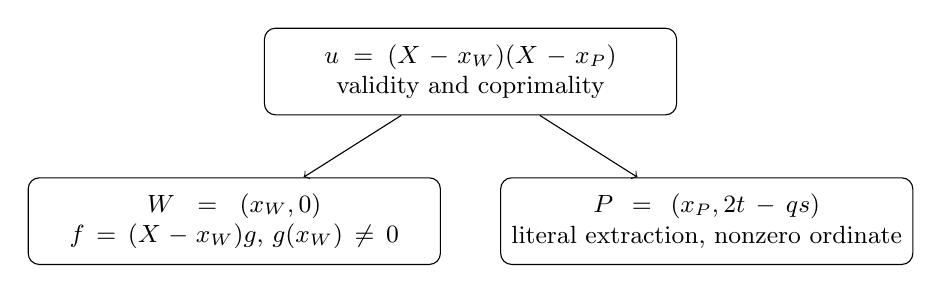
\begin{tikzpicture}[every node/.style={draw,rounded corners,align=center,text width=5cm,minimum height=1.1cm,font=\small}]
\node (s) at (0,0) {$u=(X-x_W)(X-x_P)$\\validity and coprimality};
\node (w) at (-3,-1.9) {$W=(x_W,0)$\\$f=(X-x_W)g$, $g(x_W)\ne0$};
\node (p) at (3,-1.9) {$P=(x_P,2t-qs)$\\literal extraction, nonzero ordinate};
\draw[->] (s)--(w);\draw[->] (s)--(p);
\end{tikzpicture}\end{center}
\subsection*{Binding to the weighted source branch}
The weighted theorem starts from the original six coordinates, nonzero $z,w,s$, $2\ne0$, literal source $B=0$, normalized Mumford validity and $\operatorname{IsCoprime}(f,f')$. It derives the normalized branch equation and identifies $x_P,y_P$ with the literal extracted point's decoded coordinates. A separate weighted theorem supplies the simple cofactor at $x_W$ under the same hypotheses. The normalized algebra works for arbitrary field polynomials; no quintic specialization is needed there.

This formalizes polynomial and point data used by the retained written Weierstrass argument. It does not prove valuations of principal divisors or the Jacobian class equality $2D=2P$. Those remain separate obligations. No timing, operation-count or cohort claim is made.
\subsection*{Fixed controls}
Over $\mathbf F_5$, weighted input $(q,r,s,t,z,w)=(1,0,4,0,2,3)$ normalizes to $u=X^2-X$, $v=X$ on $f=X^5+X^2-X$. The complete weighted theorem gives $W=(0,0)$ and $P=(1,1)$. The cofactor is $g=X^4+X-1$, with $g(0)=4\ne0$. The original validity witness and explicit Bezout certificate are reused verbatim from the retained fixture module.

For the singular rational example $f=X^5,u=X^2,v=X$, both support roots are zero and coprimality fails. With $(q,r,s,t)=(0,1,1,0)$ over $\mathbf Q$, the normalized branch equation is nonzero and the proposed zero-root factorization is false. Eight new fixed propositions check the positive construction and these boundaries.
\subsection*{Evidence and next task}
Named declarations, separate axiom readback, command receipts, source digests and local pre/post input bindings accompany the report. \texttt{status.json} records exact check outcomes and pending review; \texttt{control-data.json} contains typed fixtures. An unavailable root-divisibility library identifier caused one retained failed attempt; the final proof obtains divisibility directly from the previously checked extraction theorem. Control attempts also retained a name ambiguity and two heartbeat failures; explicit qualification and simplification of a rational fixture resolved them. The editable diagram is \texttt{flow.svg}.

Source: retained \texttt{PROOF\_AUDIT.md}, same-$u$ equal-$v$ doubling section, and \texttt{projective\_law\_gate.rs} lines 727--753; existing BZero, MixedCancellation and coprimality lemmas. Next: independently review these geometric bridges before extending the divisor-class proof.
\end{document}
